\chapter{Metodology}
\label{chap:Metodology}


\section{System Model}
\label{sec:control_model}

ilustramos o processo com a Figura \ref{fig:control_model_fig}. 

\begin{figure}[thpb]
  \centering
  \resizebox{150mm}{!}{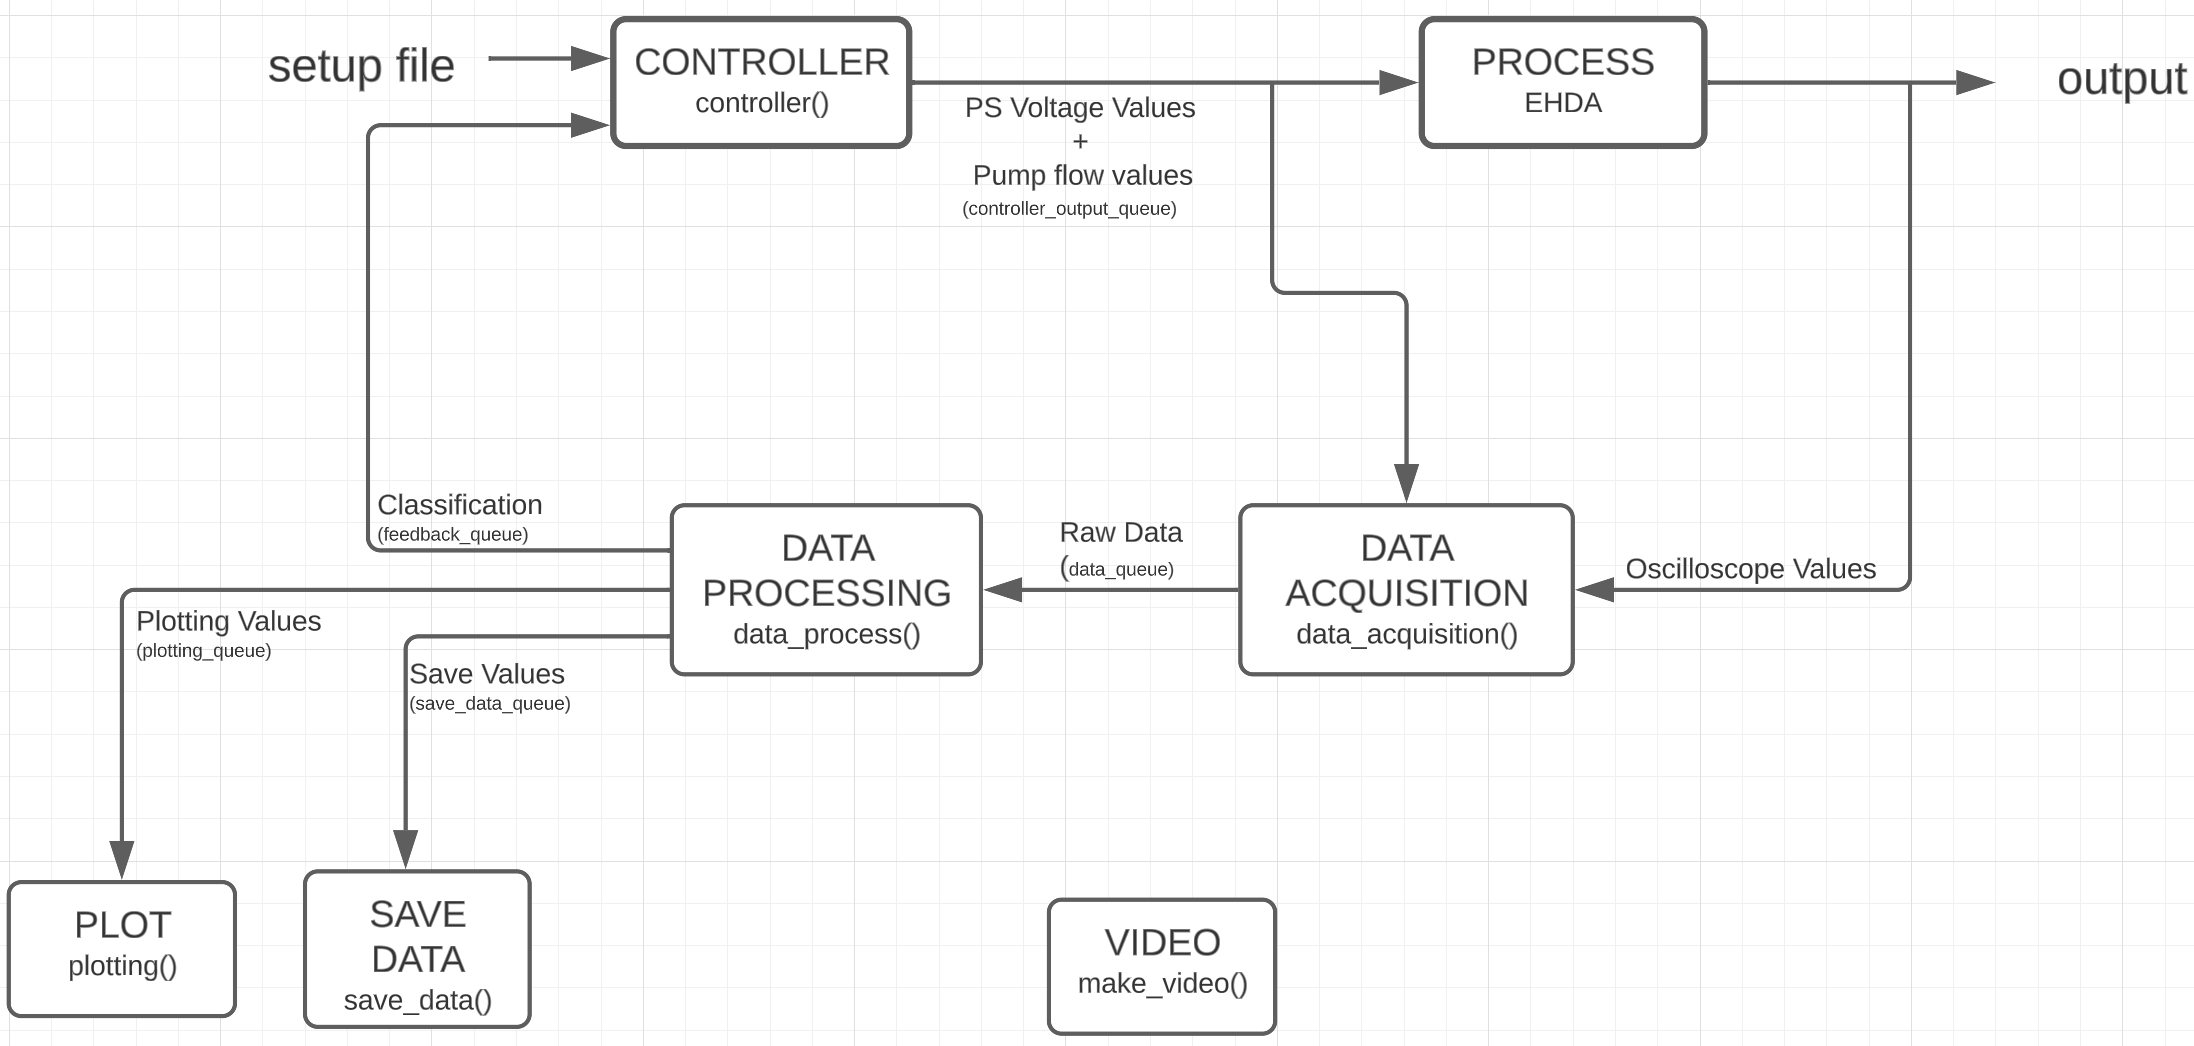
\includegraphics{Metodology/Figuras/control_loop.png}}
  \caption{EHDA automation system setup}
  \label{fig:control_model_fig}
\end{figure}

\section{Threading and Queues}
\label{sec:concurrency}

\section{Routine Sequences}
\label{sec:routine_sequences}

\subsection{Ramp}

\subsection{Step}



\subsection{Map}

\subsection{Control}

\section{Optimizations}
\label{sec:routine_optimization}

About the python algorithm to turn the experiment autonomous it was made a study and modelling of the software architecture to optimize it for further control loop application to be implemented. From the changes made until now it highlights:

- Integrate high speed camera to the experiment routine.

- Remodel the software to support threads in order to separate the sensoring and controlling routines.

- Reduce the data collected size.

- Synchronize the power supply step commands and voltage sensoring.

- Reestructure the setup file in order to make it more intuitive to use the experiment.

- Improvements in code organization and readability.

About the setup,integrate was changed the liquid, nozzle diameter and distance to the plate in order to
make the experiment the most stable and easy to reach cone-jet mode as possible. For example, while doing experiments we discovered that the frequency of the pump machine internal motors was creating an interference in the flowrate. Therefore compromising the stabilization in cone jet mode. A solution for that was to increasethe flowrate wich smooths this pumping noise. For that was also necessary to increase the nozzle diameter to balance with all other variables from the experiment.

\clearpage